\section{Environment setup and basic results}
\label{section:results}

In order to run the Wireguard in the test environment first one needs to
checkout the Wireguard package from GitHub. Thus, on each peer perform the 
following command:

\begin{verbatim}
dmitriy@initiator:~$ cd ~/
dmitriy@initiator:~$ git clone https://github.com/dmitriykuptsov/wireguard.git
\end{verbatim}

Then one needs to generate a pair of X25519 EC keys:

\begin{verbatim}
dmitriy@initiator:~$ cd wireguard
dmitriy@initiator:~$ python3 tools/genkey.py
\end{verbatim}

Copy the keys and save then in config/configuration.txt file. Also in this file modify the 
peer address (address visible on the Internet or Local Area Network (LAN) address which will be used for 
port forwarding if you are behind the network address translator (NAT)), UDP port number, and local
address of Tunneling interface (this will be used in Wireguard routing process). 

Once the file is modified on both sides you can run the Wireguard daemon as follows:

\begin{verbatim}
dmitriy@initiator:~$ sudo python3 wg.py
\end{verbatim}

Bellow we assume that peer A has 10.1.1.5 as TUN interface address, while peer B has 10.1.1.6.
We also assume that peer A's public key is $8aW8c...ZBkE=$ (of course this is a shorten version), 
while peer B has $mRpAN...KHG4=$. Run the following commands on peer A:

\begin{verbatim}
dmitriy@initiator:~$ sudo ip route add 10.1.1.0/24 via 10.1.1.5
\end{verbatim}

Then on peer B:

\begin{verbatim}
dmitriy@initiator:~$ sudo ip route add 10.1.1.0/24 via 10.1.1.6
\end{verbatim}

Add cryptographic routing entry, for that connect to WG daemon using {\it   nc} utility as follows:

\begin{small}
\begin{verbatim}
dmitriy@initiator:~$ nc -vv localhost 10000
\end{verbatim}
\end{small}

Then copy the routing entry (of course you should change the parameters that match your setting),
and press Enter key:

\begin{small}
\begin{verbatim}
add route 10.1.1.6 255.255.255.255 mRpAN...KHG4= 14501 192.168.64.19
\end{verbatim}
\end{small}

Repeat the same procedure on the other side - peer B:

\begin{small}
\begin{verbatim}
add route 10.1.1.0 255.255.255.0 8aW8c...ZBkE= 14500 192.168.64.16
\end{verbatim}
\end{small}

Now go to peer A and test the connectivity between the nodes:
\begin{verbatim}
dmitriy@initiator:~$ ping 10.1.1.6
PING 10.1.1.6 (10.1.1.6) 56(84) bytes of data.
64 bytes from 10.1.1.6: icmp_seq=1 ttl=64 time=5.77 ms
64 bytes from 10.1.1.6: icmp_seq=2 ttl=64 time=5.16 ms
\end{verbatim}

Once the secure tunnel is established you should see the ICMP packets flowing back and forth.

To understand the performance of our proof-of-concept implementation using Python language we 
have performed a series of throughput tests (with the help of the Iperf tool). All in all, 
we have reached the maximum of 70Mb/s between a pair of virtual machines hosted on a MacBook 
M1 laptop.

%\begin{figure}[!hbt]\centering
%  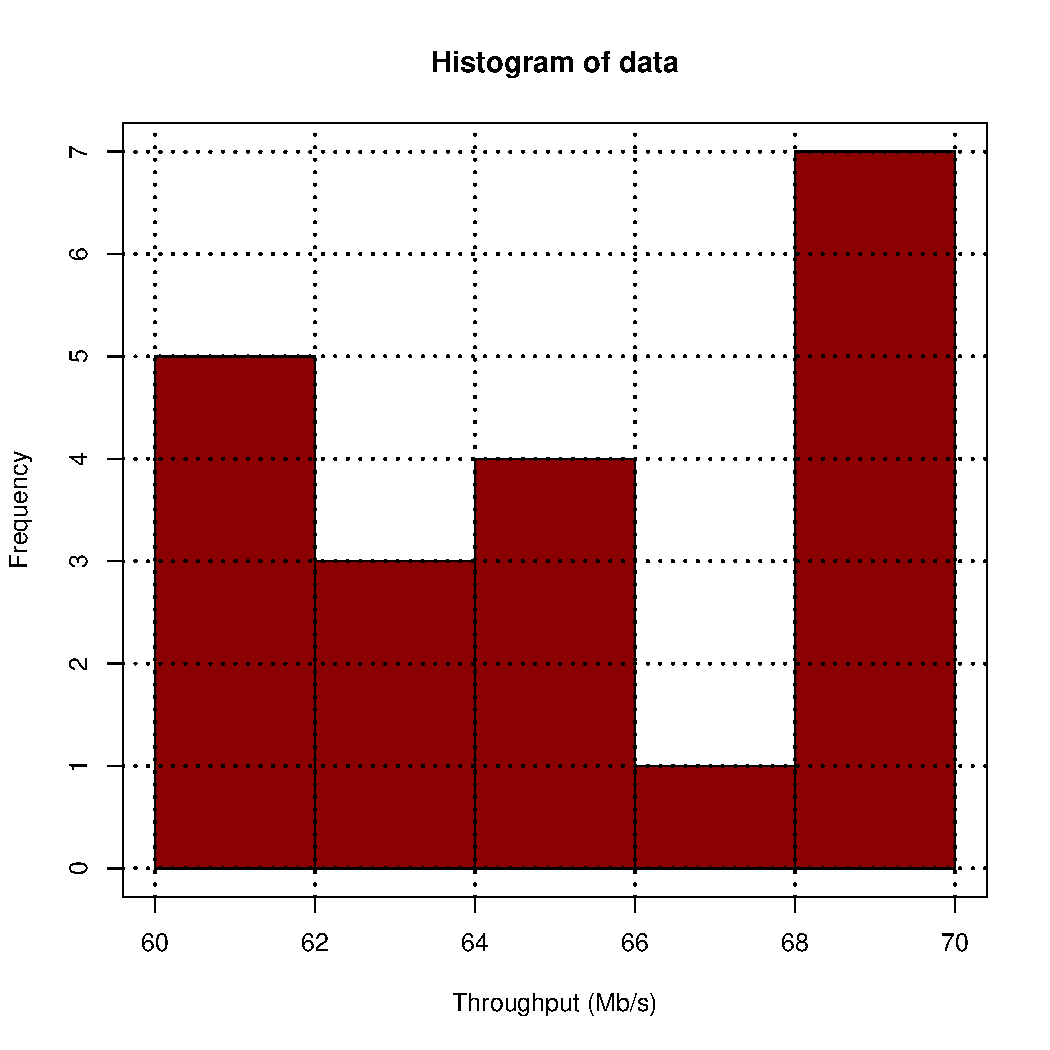
\includegraphics[width=0.45\textwidth]{graphics/throughput.pdf}
%  \caption{Distribution of throughput}
%  \label{fig:throughput}
%\end{figure}
